% ============================================================
% 第二章 系统需求分析与总体方案
% ============================================================

\chapter{系统需求分析与总体方案}

\section{应用场景分析与使用流程设计}

\subsection{目标应用场景}

飞行雨伞系统的核心应用场景定位于私家车用户的日常城市出行——
具体指用户驾车抵达目的地停车后、步行前往目的建筑物这一段
"最后数十米"的室外步行过程。这一场景具有以下典型特征：
其一，发生频率高，几乎涵盖所有有驾车出行需求的用户的日常生活；
其二，空间条件受限，用户通常处于停车场、街道或广场等开阔或半开阔环境，
无遮蔽设施；其三，天气敏感性强，雨天、烈日等恶劣气候条件下
用户对遮护需求最为迫切；其四，用户双手通常处于携带物品状态，
难以同时操持传统雨伞。

上述场景特征决定了飞行雨伞系统的几个核心设计约束：
系统必须以车辆为部署基点，能够快速展开、无需手持、
自主悬停于用户上方，并在任务结束后安全归位收纳。

% ----------------------------------------------------------
% [图片占位 Fig.2.1] ★需要制作★
% 内容：目标应用场景示意图
%   示意图包含：停车场/街道背景、用户步行图示、飞行雨伞悬停于头顶上方
%   可使用效果渲染图或手绘场景示意图
%   也可使用第六章中的那张概念效果图（generated-image-4.jpg）
% \begin{figure}[htbp]
%     \centering
%     \includegraphics[width=0.80\textwidth]{figures/fig2_1_scenario.png}
%     \caption{飞行雨伞目标应用场景示意图}
%     \label{fig:scenario}
% \end{figure}
% ----------------------------------------------------------

\subsection{使用流程设计}

基于对目标场景的分析，飞行雨伞系统的使用流程设计共分六个阶段，
如图~\ref{fig:workflow}所示：

\begin{description}
    \item[阶段一：收纳待机（Storage Standby）]
        系统以排气折叠状态固定于车顶或车尾专用车载平台上。
        充气结构完全压缩，整体占用空间极小，不影响车辆正常行驶与停放。

    \item[阶段二：充气展开（Inflation \& Deployment）]
        用户触发启动指令后，车载充气设备启动，向气囊充气。
        充气伞形结构在设计时间内完成展开，达到飞行所需的结构刚度与气动形态。
        此阶段系统仍固定于车载平台，尚未起飞。

    \item[阶段三：起飞（Takeoff）]
        充气展开确认完成后，多旋翼动力系统启动，飞行器从车载平台垂直起飞，
        上升至设计悬停高度（距地面约$2.0\sim2.5$\,m）。

    \item[阶段四：遮雨服务（Shelter Mode）]
        飞行器在用户头顶上方设计高度悬停，充气伞面提供有效遮雨遮阳防护。
        此阶段为系统的核心服务阶段，飞行器保持位置稳定悬停，用户可自由步行移动。
        本阶段的用户跟随功能（基于视觉或UWB定位）属于未来扩展方向，
        本文实现的是固定位置悬停验证。

    \item[阶段五：降落归位（Landing \& Return）]
        服务完成后，用户触发降落指令，飞行器垂直降落回车载平台起降区，完成归位。

    \item[阶段六：排气收纳（Deflation \& Storage）]
        飞行器降落并固定后，排气阀开启，气囊排气，
        充气结构折叠回收纳态，系统恢复待机状态。
\end{description}

以上六个阶段构成飞行雨伞系统的完整工作闭环，
也是本文后续各章节技术设计的总体逻辑主线。

% ----------------------------------------------------------
% [图片占位 Fig.2.2] ★需要制作★
% 内容：六阶段使用流程图（横向时序图）
%   六个阶段从左到右排列，每个阶段一个方框+简短文字+小图标
%   阶段间用箭头连接，整体呈线性流程图样式
%   建议用PowerPoint或draw.io绘制
% \begin{figure}[htbp]
%     \centering
%     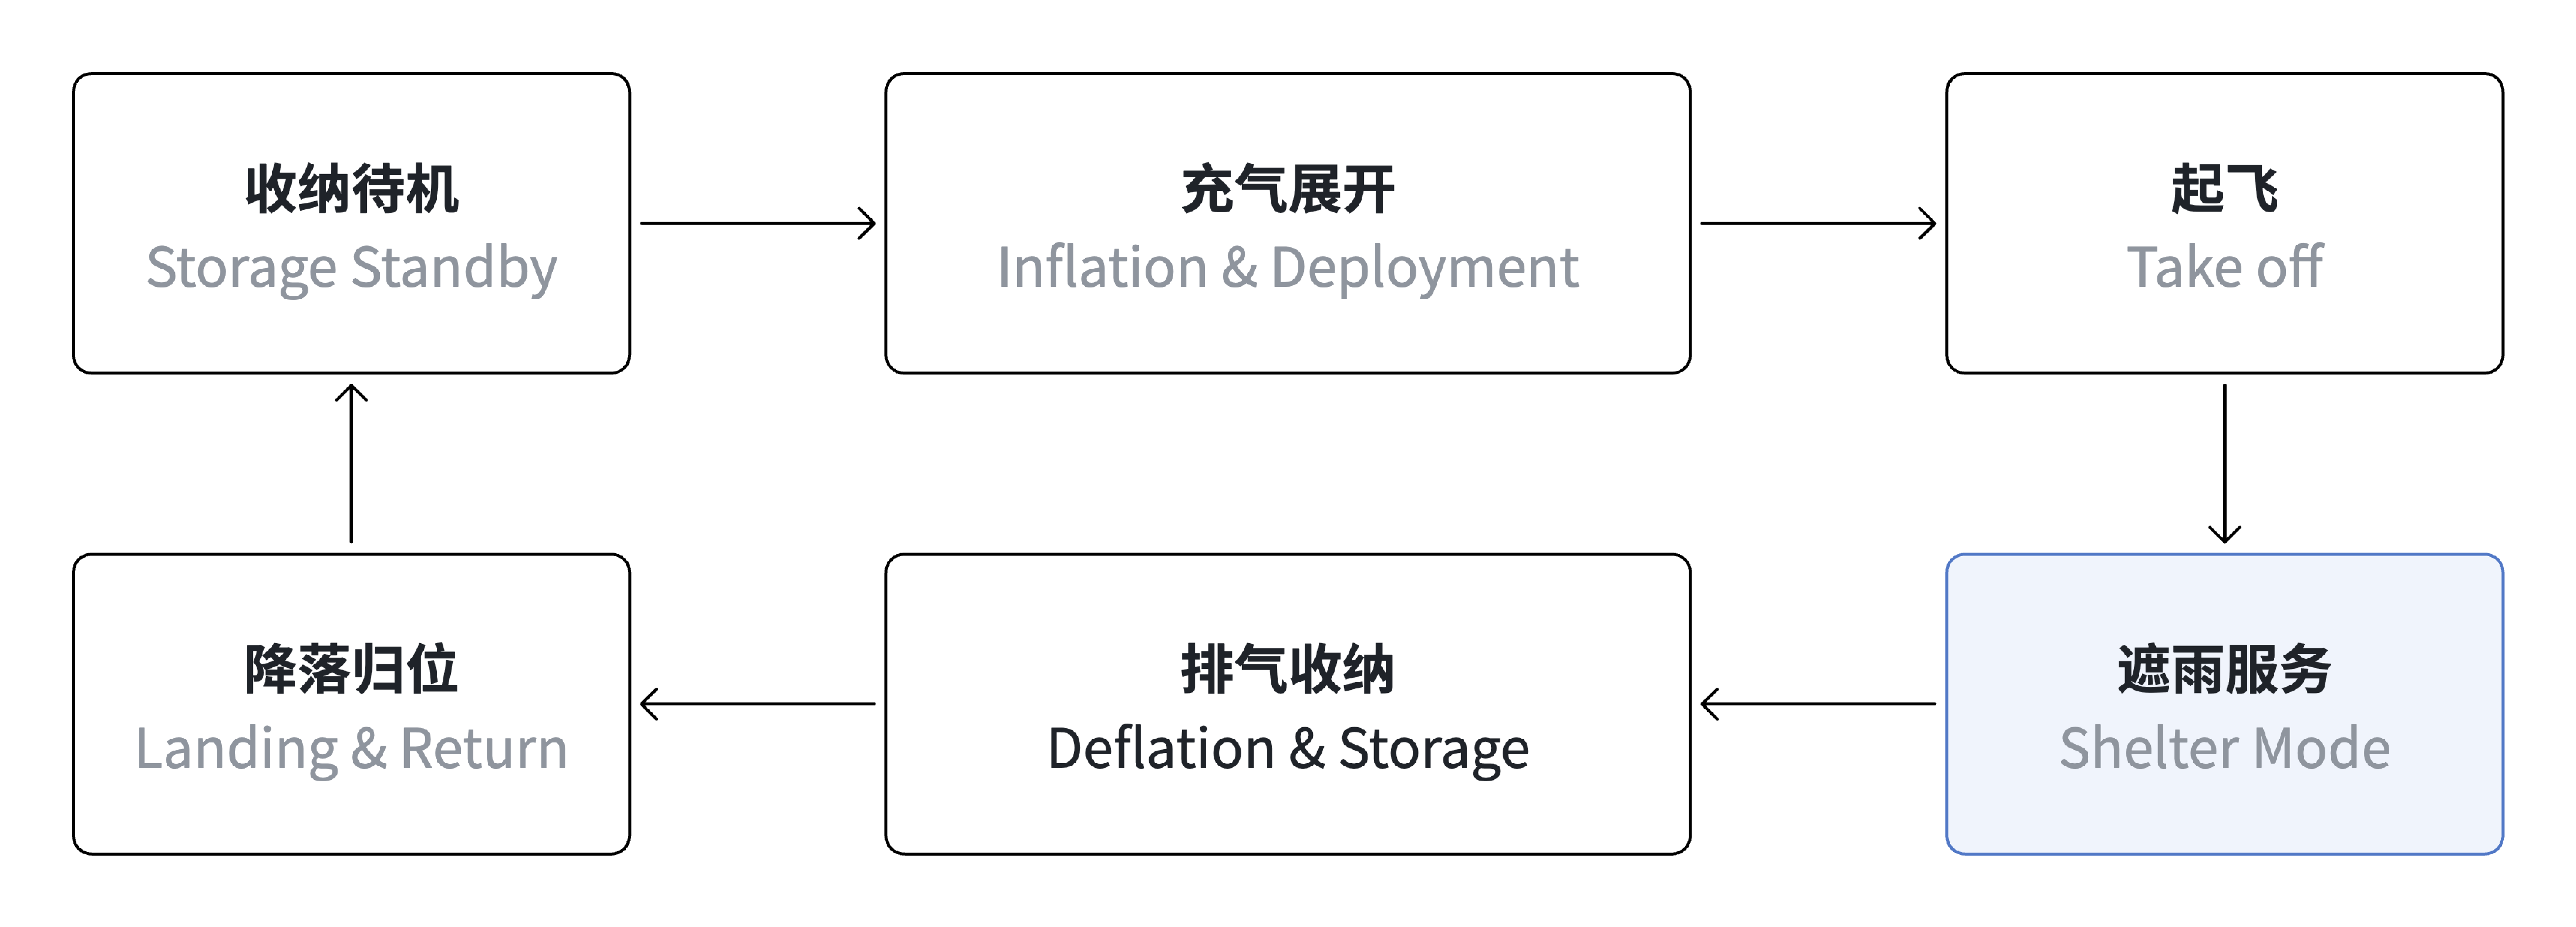
\includegraphics[width=\textwidth]{figures/fig2_2_workflow.png}
%     \caption{飞行雨伞系统六阶段使用流程图}
%     \label{fig:workflow}
% \end{figure}
% ----------------------------------------------------------

\subsection{供电形态设计}

结合实际使用需求，飞行雨伞系统设计了两种互补的供电形态，以适应功能验证与实际出行场景的不同需求，
如表~\ref{tab:power_mode}所示。

\begin{table}[htbp]
    \centering
    \caption{两种供电形态对比}
    \label{tab:power_mode}
    \begin{tabular}{lll}
        \toprule
        对比维度         & 自载电池模式               & 系留供电模式 \\
        \midrule
        供电来源         & 机载6S 1500\,mAh电池       & 地面6S 10000\,mAh电池（有线） \\
        理论续航         & 约3\,min（应急用途）        & $\geq15$\,min \\
        飞行自由度       & 完全无线，机动性强           & 受系留缆线约束（缆长约150\,cm） \\
        用户双手         & 不影响                     & 电源可入包/入口袋，双手完全解放 \\
        主要用途         & 功能验证、自主返航备用电源    & 日常遮雨服务、长时悬停任务 \\
        安全冗余         & 独立供电，无断连风险          & 缆线物理拉力防止失控高飞 \\
        \bottomrule
    \end{tabular}
\end{table}

\textbf{自载电池模式（Onboard Battery Mode）}：
飞行雨伞搭载机载小电池（样机为6S 1500\,mAh），系统完全自主、无线缆束缚。
该模式主要服务于两个场景：一是早期功能验证与短时飞行测试；
二是在系留模式主电源意外断连时，机载电池作为应急备用电源，
为系统提供足够完成一次安全降落或自主返航的动力裕量，有效规避炸机风险。
由于机载电池容量较小，该模式不作为日常服务的主要供电方式。

\textbf{系留供电模式（Tethered Power Mode）}：
飞行器通过轻质供电线缆与地面大容量电池（样机为6S 10000\,mAh）有线连接，
彻底解除了机载电池容量对续航的限制。
地面电源可由用户随身携带（置于背包或裤兜），无需手持，真正实现双手解放。
系留缆线设计长度约150\,cm，满足飞行雨伞在约2\,m悬停高度下的运动自由度，
并在测试阶段通过缆线末端的物理拉力提供额外安全冗余，防止失控高飞。
系留模式是飞行雨伞面向实际出行场景的主要工作形态。

两种供电形态通过插拔电源接口实现快速切换，相互补充，
共同构成飞行雨伞系统完整的能源管理方案。


\section{功能需求与关键性能指标}

\subsection{功能需求分解}

根据使用流程分析，飞行雨伞系统需满足以下核心功能需求：

\begin{itemize}
    \item \textbf{形态重构能力：}系统须能在收纳态与飞行态之间实现可靠的双向切换，
          充气展开过程自动完成，无需人工干预；
    \item \textbf{飞行稳定性：}飞行器需在有效载荷（充气伞体）条件下实现稳定悬停，
          姿态偏差满足服务要求；
    \item \textbf{遮雨有效性：}充气伞面展开后需提供足够的遮蔽面积，
          能够有效覆盖单人的头部及肩部区域；
    \item \textbf{车载适配性：}系统收纳态尺寸需适配车顶或车尾安装空间，
          固定方案安全可靠，不影响车辆正常使用；
    \item \textbf{操作便捷性：}从用户发出指令到飞行器完成起飞悬停的全程时间
          应控制在合理范围内，满足实际出行场景的时间容忍度。
\end{itemize}

\subsection{关键性能指标体系}

基于功能需求，结合工程可行性分析，制定本系统的关键性能指标（KPI）如表~\ref{tab:kpi}所示。

\begin{table}[htbp]
    \centering
    \caption{飞行雨伞系统关键性能指标}
    \label{tab:kpi}
    \begin{tabular}{llll}
        \toprule
        指标类别       & 指标项目         & 设计目标值              & 验证方式 \\
        \midrule
        \multirow{3}{*}{飞行性能}
                      & 悬停稳定性       & 姿态偏差 $\leq \pm5°$   & 飞控日志分析 \\
                      & 推重比           & $\geq 1.5$             & 动力计算+测试 \\
                      & 最大工作高度     & $2.0\sim2.5$\,m        & 实飞验证 \\
        \midrule
        \multirow{2}{*}{续航性能}
                      & 系留模式续航     & $\geq 15$\,min          & 实飞计时 \\
                      & 自载模式续航     & $\geq 3$\,min（应急）   & 实飞计时 \\
        \midrule
        \multirow{2}{*}{遮护性能}
                      & 伞面遮蔽面积     & $\geq 0.40$\,m$^2$      & 几何测量 \\
                      & 防水等级         & 有效阻断垂直降雨         & 功能验证 \\
        \midrule
        \multirow{3}{*}{形态重构}
                      & 充气展开时间     & $\leq 60$\,s            & 计时测试 \\
                      & 排气收纳时间     & $\leq 60$\,s            & 计时测试 \\
                      & 收纳后尺寸       & 厚度 $\leq 5$\,cm       & 实物测量 \\
        \midrule
        \multirow{2}{*}{系统集成}
                      & 起飞准备时间     & $\leq 90$\,s            & 全流程计时 \\
                      & 整机起飞质量     & $\leq 2.0$\,kg（不含地面电源）& 称重 \\
        \bottomrule
    \end{tabular}
\end{table}

上述指标将作为后续各章节设计计算的约束条件与验证基准。
部分指标（如悬停续航时间）将在实验验证章节与理论估算值进行对比分析。


\section{方案论证}

\subsection{充气方案与刚性方案对比分析}

对于实现"可收纳大面积飞行遮护结构"，在工程上有两种基本技术路线：
充气结构方案与刚性折叠结构方案。两种方案的主要特性对比如表~\ref{tab:scheme_compare}所示。

\begin{table}[htbp]
    \centering
    \caption{充气结构方案与刚性折叠方案对比}
    \label{tab:scheme_compare}
    \begin{tabular}{lll}
        \toprule
        对比维度       & 充气结构方案                     & 刚性折叠结构方案 \\
        \midrule
        收纳体积       & 极小（排气后近似零体积）          & 较大（折叠比约1:3$\sim$1:5） \\
        展开方式       & 充气自动展开，操作简单            & 机械铰链折叠，需人工/电动展开 \\
        系统重量       & 轻（气囊薄膜面密度低）           & 重（碳纤维/金属骨架） \\
        结构刚度       & 依赖充气压力，有一定限制          & 高刚度，结构可靠性强 \\
        制作难度       & 低（标准气柱+3D打印节点）        & 高（折叠机构设计加工复杂） \\
        失效模式       & 漏气导致刚度下降                 & 铰链卡死/疲劳断裂 \\
        维修成本       & 低（气柱可替换）                 & 高（金属/碳纤维件加工成本高） \\
        \bottomrule
    \end{tabular}
\end{table}

综合以上对比，充气结构方案在收纳体积、系统重量与制作工艺三个维度上具有明显优势，
与本系统对车载收纳便捷性与轻量化的核心需求高度契合。
刚性折叠方案虽在结构可靠性上略有优势，
但其难以突破的收纳尺寸下限使其无法满足本系统的收纳性能指标。
因此，本文选择充气结构方案作为伞体形态重构的实现路径。

\subsection{旋翼布局方案选型}

多旋翼飞行器的旋翼布局方案直接影响系统的飞行稳定性、控制解耦性与结构集成难度。
针对飞行雨伞系统的伞形载体特征，对以下三种主流布局方案进行分析与比较，
如表~\ref{tab:rotor_compare}所示。

\begin{table}[htbp]
    \centering
    \caption{三种旋翼布局方案对比}
    \label{tab:rotor_compare}
    \begin{tabular}{llll}
        \toprule
        布局方案              & 优势                        & 劣势                     & 适配性评估 \\
        \midrule
        四旋翼X型（标准）     & 控制成熟、开源支持完善       & 抗非对称干扰能力一般      & 中等 \\
        六旋翼（Y6/六轴）     & 冗余度高、抗扰能力强         & 重量增加、结构复杂        & 较低 \\
        四旋翼伞缘分布式      & 伞体即机臂、结构一体化       & 控制与普通四旋翼一致      & \textbf{最优} \\
        \bottomrule
    \end{tabular}
\end{table}

四旋翼伞缘分布式布局将旋翼直接安装于充气伞形结构的周缘，
利用伞体结构本身作为机臂替代，可最大化利用伞形空间并降低系统质心高度。
这是本项目最具针对性的布局方案，也是充气伞形结构的自然几何约束给出的最优解。
同时，四旋翼布局继承了标准四旋翼完善的PX4飞控支持，
降低了控制系统的开发门槛。
综合考虑控制成熟度、结构重量与对本系统伞形载体的适配性，
本文选择\textbf{四旋翼伞缘分布式布局}作为动力系统布局方案。
旋翼具体安装位置与重心匹配分析将在第四章详细展开。


\section{系统总体架构}

飞行雨伞系统由四个子系统组成，各子系统相互协同，共同支撑完整工作流程的实现。

% ----------------------------------------------------------
% [图片占位 Fig.2.3] ★需要制作★
% 内容：系统总体架构图（四个子系统的关系框图）
%   四个方框：充气伞体系统、多旋翼动力系统、嵌入式飞控系统、车载平台系统
%   用双向箭头或单向箭头表示子系统间的能量/信号/结构依赖关系
%   建议用draw.io或PowerPoint绘制
% \begin{figure}[htbp]
%     \centering
%     \includegraphics[width=0.80\textwidth]{figures/fig2_3_architecture.png}
%     \caption{飞行雨伞系统总体架构图}
%     \label{fig:architecture}
% \end{figure}
% ----------------------------------------------------------

\subsection{充气伞体系统}

充气伞体系统是本项目的核心创新载体，承担形态重构与遮雨防护两项核心功能。
该子系统包括：气囊本体（薄壁气柱，构成伞形骨架与遮护面）、
PLA节点连接件（维持伞形几何形态）、
充气接口（与充气子系统对接）、
以及TPU伞面（提供遮雨遮阳功能）。
充气伞体系统的详细设计见第三章。

\subsection{多旋翼动力系统}

多旋翼动力系统为飞行器提供垂直升力与姿态控制所需的力矩输出，
由四组无刷电机（SIRIUS 2306.5-1850KV）、
电子调速器（ESC）、桨叶（51366 MCK v3）
与供电系统（机载电池或地面系留电源）组成。
动力系统的选型基于整机质量预算与悬停升力需求的理论计算结果，
具体计算过程见第四章。

\subsection{嵌入式飞行控制系统}

嵌入式飞行控制系统以Pixhawk 6C开源飞控为核心计算平台，
搭载NuttX实时操作系统，集成IMU（惯性测量单元）、气压计、磁力计等传感器，
负责完成传感器数据融合、姿态估计、飞行控制律解算与电机PWM指令输出。
PX4固件提供了成熟的多旋翼姿态控制回路与位置控制回路，
是系统实现稳定悬停的核心保障。飞控系统架构与参数整定过程见第五章。

\subsection{车载平台系统}

车载平台系统承担系统的部署基础功能，包括：
承载结构（固定于车顶行李架或车尾的安装基板）、
起降区域（为飞行器提供标定的起飞与降落落点）、
充气设备（车载12\,V微型气泵，通过快接接口与气囊连接）、
以及电源接口（通过车载12\,V电源为充气设备供电）。
车载平台的详细设计见第六章。


\section{本章小结}

本章从应用场景出发，完成了飞行雨伞系统的需求分析与总体方案设计。
通过对目标场景的系统梳理，提出了涵盖六个阶段的完整使用流程，
并在此基础上设计了自载电池与系留供电两种互补的供电形态，
以适应功能验证与实际使用场景的不同需求。
本章建立了系统关键性能指标体系，并通过充气方案与刚性方案的对比论证、
旋翼布局的选型分析，确定了本系统的核心技术路线。
在此基础上，提出了由充气伞体系统、多旋翼动力系统、
嵌入式飞行控制系统与车载平台系统四个子系统构成的总体架构，
为后续各章节的详细设计提供了清晰的工程框架。